\documentclass{article}

\title{Information choice and state uncertainty}
\author{Cameron Pfiffer}

\usepackage{palatino}
\usepackage{amsmath}
\usepackage{todonotes}
\usepackage{optidef}
\usepackage{color,soul}
\usepackage{physics}
\usepackage{graphicx}
\usepackage{caption}
\usepackage{subcaption}
% \setlength{\parindent}{0pt}

\hfuzz=20pt 

\if@todonotes@disabled
    \newcommand{\hlfix}[2]{#1}
    \else
    \newcommand{\hlfix}[2]{\texthl{#1}\todo{#2}}
\fi

\usepackage[style=apa, 
backend=biber, 
giveninits=true,
uniquelist=false, 
uniquename=init,
isbn=false, 
maxcitenames=2,
dashed=false, 
maxbibnames=999,
doi=false,
url=false]{biblatex}
\addbibresource{bibs/library.bib}

\begin{document}

% Shortcut variables
\newcommand{\Gauss}{\mathcal{N}}
\newcommand{\Var}{\text{Var}}
\newcommand{\E}{\text{E}}
\newcommand{\argmax}{\text{argmax}}

% Theorem styles
\newtheorem{definition}{Definition}


Stochastic variables:

\begin{itemize}
    \item State variable $s ~ \sim \text{Bernoulli}(\pi)$. $P(s=H) = \pi$, $P(s=L) = 1-\pi$.
    \item Risk factor payoffs $\tilde f \mid s \sim N(\Gamma^{-1} \mu_s, \Sigma_s)$
    \item Risk factor supply $x \sim N(\overline{x}, \sigma_x I)$
    \item Private signals $\eta_j \mid s \sim N(z, \Sigma_{\eta_j})$
    \item Price signal $\eta_p \mid s \sim N(z, \Sigma_p)$
\end{itemize}

Joint density:

$$
P(s, \tilde f, x, \eta_j, \eta_p) = P(\tilde f \mid s) P(\eta_j \mid s) P(\eta_p \mid s) P(s)  P(x)
$$

Posterior density:

$$
P(s, \tilde f \mid x, \eta_j, \eta_p) = 
    \frac{
        P(x, \eta_j, \eta_p \mid s, \tilde f) P(s, \tilde f)
    }{
        P(x, \eta_j, \eta_p)
    }
$$

Unknown values:

\begin{itemize}
    \item $E_j[\tilde f - \tilde p r \mid H]$
    \item $E_j[\tilde f - \tilde p r \mid L]$
    \item $V_j[\tilde f - \tilde p r \mid H]$
    \item $V_j[\tilde f - \tilde p r \mid L]$
    \item $P(H \mid \eta_p, \eta_j)$
    \item $P(L \mid \eta_p, \eta_j)$
    \item $E_j[\tilde f \mid \eta_p, \eta_j]$
    \item $V_j[\tilde f \mid \eta_p, \eta_j]$
    \item $\tilde p$
\end{itemize}

Portfolio choice problem:

\begin{align*}
    U_{2j} &= \max_{\tilde q_j}
        \rho E_j [W_j] - \frac{\rho^2}{2} V_j [W_j] \\
\end{align*}

Optimal quantity:

\begin{align*}
    \tilde q_j &= \frac1\rho \bigg( P(H) \Sigma_H + P(L) \Sigma_L \bigg)^{-1} \bigg(
        P(H) E_j [\tilde f \mid H] + P(L) E_j [\tilde f \mid L] - \tilde p r
    \bigg) \\
    &= \frac1\rho V_j[\tilde f]^{-1} (E_j [\tilde f] - \tilde p r)
\end{align*}

Ex-ante expected utility:

\begin{align*}
    U_{1j} &= E\biggl[
        \rho E_j [W_j] - \frac{\rho^2}{2} V_j [W_j]
    \biggr] \\
    &= 
        \pi E\biggl[
            \rho E_j [W_j \mid H] - \frac{\rho^2}{2} V_j [W_j \mid H]
        \biggr] \\
        &\quad +
        (1-\pi) E\biggl[
            \rho E_j [W_j \mid L] - \frac{\rho^2}{2} V_j [W_j \mid L]
        \biggr] \\
    &= \rho r W_0 \\
        &\quad + 
        \rho \tilde q'_j \biggl(
            \pi E_j [\tilde f - \tilde p r \mid H] +
            (1-\pi) E_j [\tilde f - \tilde p r \mid L]
        \biggr) \\
        &\quad -
        \frac{\rho^2}{2} \tilde q'_j \biggl(
            \pi V_j [\tilde f - \tilde p r \mid H] +
            (1-\pi) V_j [\tilde f - \tilde p r \mid L]
        \biggr) \tilde q_j
\end{align*}

\newpage

\maketitle

\section{Introduction}

A strand of economic literature studies how limited attention and cognitive constraints guide economic choices. In these papers, researchers examine how prices can be used to aggregate private signals observed by attention-constrained investors. Signals usuall\footnote{A noteworthy exception is \textcite{breon-drish_existence_2015}, which allows signals and payoff distributions to vary to a greater degree -- namely, that the density of the payoff conditional on a private signal ($P(\tilde f \mid \eta_j)$, in terms of \textcite{kacperczyk_rational_2016}) be a member of the exponential family of distributions.} take the form of the true payoff with additive Gaussian nois, $\eta_j = \tilde f + \epsilon_j$, for investor $j$, signal $\eta_j$, payoff vector $\tilde f$, and noise term $\epsilon_j$. 

I examine how endogenous information choice with attention limitations can lead investors to choose distinct portfolios when signals inform investors about both the underlying economic state and asset payoffs in those states. Allowing risk averse investors to select signals that are informative about state and payoffs jointly produces \hl{substantially different} \todo[noline]{Check if this actually happened} portfolios from standard noisy rational equilibrium models, as well as shifting the conclusions of canonical models of information choice where signals inform investors \textit{only} about payoffs.

\todo{lit review here}

\section{Model framework}

Much of my notation and model structure follows from \textcite{kacperczyk_rational_2016},  which introduce attention constraints and information choice to the multiasset noisy rational equilibrium model of \textcite{admati_noisy_1985}.

The model has three periods. In time 1, informed investors allocate their attention across $n$ signals. At time 2, all investors construct portfolios. At time 3, all investors receive payoffs.

I assume, as in \textcite{kacperczyk_rational_2016}, that there are $n$ risky assets with an arbitrary factor structure given by principal components. Assets $1,2,\dots,n$ represent specific assets with idiosyncratic shocks. The key difference between my paper and \textcite{kacperczyk_rational_2016} is that the economic state is a stochastic variable that is not known by investors. The economy is in state $s \in {H, L}$, where $s=H$ represents a "good" state with probability $\pi$ and $s=L$ represents a "bad" state with probability $1-\pi$. The density of $s$ is written

$$
P(s) = \begin{cases}
    \pi & \text{ if } s = H \\
    1-\pi & \text{ if } s = L \\
\end{cases}
$$

Importantly, asset payoffs are governed by two different stochastic processes conditional on state. Payoffs of the $n$ assets are written

\begin{align}
    f_i &= \mu_{i,s} + z_i\\
    z &= [z_1,z_2, \dots, z_n]' \sim \Gauss(0, \Sigma_s) \\
    f &\mid s \sim \Gauss(\mu_{s}, \Sigma_s)
\end{align}

\noindent That is, both the mean payoff vector $\mu_s = [\mu_{1,s},\mu_{2,s},\dots,\mu_{n,s}]'$ and the  $n\times n$ variance-covariance matrix of payoff shocks $\Sigma_s$ are functions of the unobserved economic state. When investors are allowed to receive signals about the underlying shocks $z$, those same signals will allow investors to assign a probability to the underlying state and the associated payoff structure.\footnote{\textcite{kacperczyk_rational_2016} utilize a transformation of asset payoffs to the corresponding risk factor payoffs -- in my case, the eigen-decomposition $\Sigma_s = \Gamma_s \Lambda_s \Gamma_s'$ for $s \in {H,L}$ yields Arrow-Debreu synthetic securities on risk factors:

\begin{align}
    \tilde f \mid s \sim \Gauss(\Gamma_s^{-1} \mu_s, \Lambda_s)
\end{align}

\noindent Unfortunately, I cannot proceed with the \textcite{kacperczyk_rational_2016} solution method, which requires an additional transformation of risk factor prices $\tilde p = \Gamma^{-1}p$ and risk factor quantities $\tilde q = \Gamma^{-1} q$ for some eigenvector matrix $\Gamma$. My model only permits the orthogonalization of the prior variance $\Sigma$, but in general the transforms on $\tilde q$ and $\tilde p$ will remain correlated conditional on state.


}

Note that the unconditional payoff density $P(f)$ is a two-component Gaussian mixture distribution with mixture weights $\pi$ and $1-\pi$. The density function is written

\begin{align}
    P(f) \sim \pi \Gauss(f \mid \mu_H, \Sigma_H) + (1-\pi) \Gauss (f \mid \mu_L, \Sigma_L)
\end{align}

\noindent Gaussian mixture distributions have the conceptual benefit of moving payoffs outside the traditional exponential family of distributions. In principle, a mixture model with more and more components can approximate any complex joint density (\cite{nguyen_approximations_2019}). The shift towards a mixture distribution does however present some technical difficulties in that closed-form posterior distributions are not generally available.

\begin{figure}
    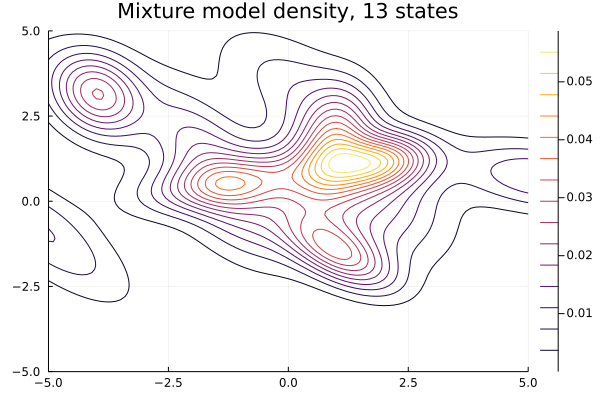
\includegraphics[width=\textwidth,height=\textheight,keepaspectratio]{plots/mixture-1.png}
    \caption{The joint density contour plot of a multimodal Gaussian mixture distribution. Dimensionality is $\mathcal{R}^2$.}
\end{figure}

As in \textcite{admati_noisy_1985} and \textcite{kacperczyk_rational_2016}, I employ CARA utility to abstract from wealth effects. However, the conditions in \textcite{kacperczyk_rational_2016} that reduce the investment problem to a mean-variance problem do not hold in my setting. Namely, the distribution of $f$ is non-Gaussian. Non-Gaussian payoffs invalidate the Taylor expansion of the utility function that is commonly employed to simplify the investment decision.

The economy is populated by atomistic investors $j$ with unit mass ($j \in [0, 1]$). Investors have exponential preferences on final-period wealth $W_j$, with a risk-aversion coefficient $\rho$. Expected utilityat time 2 (after receiving private signals) is a function of risk-free rate $r$, initial wealth $W_0$, asset quantities $q_j$, asset payoffs $f$, and asset prices $p$.

\begin{align}
    U_{j2} = E_j[\exp{-\rho W_j}]
\end{align}

\noindent for law of motion on wealth $W_j = r W_0 + q'_j (f - pr)$. Since wealth effects do not enter the investment decision for CARA utilities, I follow  \textcite{kacperczyk_rational_2016} and equalize all initial wealth to $W_0$.

A portion of investors receive private signals $\eta_j$ about time 3 payoffs $f$. Signals take the form of additive Gaussian noise around the true payoff, where the precision of the noise is determined by investor attention allocation. The form of a private signal is

\begin{align}
    \eta_j \sim \Gauss(f, \Sigma_{\eta,j})
\end{align}

\noindent The matrix $\Sigma_{\eta_j}$ is a diagonal matrix with entries $K_{ij}^{-1}$. $K_{ij}$ is a \textit{unit} of attention given to signal $i$ by investor $j$. Higher values of $K_{ij}$ imply higher precision, and thus a more accurate signal of $f$.

Investors have limited attention, in that they cannot pay attention to all the signals they would like. Concretely, this constraint is written

\begin{align}
    \sum_{i=1}^n K_{ij} \le K_j
\end{align}

\noindent though for simplicity I equalize attention constraints across investors to $K_j = K$ for informed investors and $K_j = 0$ for uninformed investors. Uninformed investors can only use prices as signals about payoffs, whereas informed investors can use both prices and private signals. The attention constraint utilized here is common in the information choice literature -- see \textcite{kacperczyk_rational_2016}.

Investors have two optimization problems to make. First, if the investor is informed, they must allocate their attention across private signals at time 1. Second, conditional on any information observed in time 1, investors construct portfolios to optimize expected utility at time 2, $U_{j2}$.

The investor's information choice problem is to maximize expected time-1 utility $U_{j1}$:

\begin{maxi}
    {K_{ij}}{U_{j1} = E\bigg[ E_j[\exp{-\rho W_j}]\bigg]}
    {\label{eq:learning-opt}}{}
    \addConstraint{W_j }{= r W_0 + q'_j (f - pr)}
    \addConstraint{\sum_i K_{ij}}{ \le 1}
    \addConstraint{K_{ij}}{\ge 0, \quad \forall i}
\end{maxi}

\noindent Next, the time-2 portfolio choice problem is to maximize expected utility $U_{j2}$:


\begin{maxi}
    {q_{j}}{U_{j2} = E_j[\exp{-\rho W_j} \mid \eta_j, p]}
    {\label{eq:learning-opt}}{}
    \addConstraint{W_j }{= r W_0 + q'_j (f - pr)}
\end{maxi}

Finally, markets must clear at price $p$ and quantities $q_j$, leading to the traditional market clearing condition

\begin{align}
    \int_j{q_j(p)} = \overline x + x
\end{align}

\noindent Market clearing requires that quantities and prices be such that all supply is allocated to an investor. I now turn to the formal declaration of an equilibrium in my setting, as in \textcite{breon-drish_existence_2015}.

\begin{definition}
    A noisy rational expectations equilibrium (NREE) is a function $p(s, f, x)$ that maps the state $s$, payoffs $f$, and asset supply $x$ to a vector of prices for the $n$ assets, such that (a) prices maximize aggregate surplus:

    \begin{align}
        q_j(p, \eta_j) \in \arg\max_{q_j} E_j [\exp{-\rho W_j} \mid \eta_j, p], \quad \forall j \in [0,1]
    \end{align}

    \noindent that (b) markets clear, and (c) that all agents are optimizing conditional on their information set $\{p, \eta_j\}$.

\end{definition}

The history of the price function in noisy rational equilibrium models is an interesting one. Traditionally, generating the pricing function reduces to conjecturing that $p$ is Gaussian because it is a linear combination of Gaussians (payoffs $f$ and supply shocks $x$) as in \textcite{admati_noisy_1985}. Others have broadened the concept of the price as a distribution to allow for non-Gaussian payoffs such as \textcite{breon-drish_existence_2015}. \textcite{breon-drish_existence_2015} removed the limitation with non-Gaussian payoffs as long as the density is in the exponential family of distributions. 

I seek to describe the properties of the joint density $P(p, z, x, s, \eta_j)$ so as to reduce the problem of finding a price that rationalizes a NREE. I conjecture that the price function $p$ is additive in functions on the payoff and state variables ($\psi(f, s)$) and in the supply shocks ($\phi(x)$).

\begin{align}
    p(s,f,x) = A + \psi(f, s) + C x
\end{align}

\noindent for $n \times 1$ vectors $A$ and $\psi(f,s)$. I conjecture that $p$ is strictly a linear function in $x$, since $x$ is Gaussian. The most complex portion of the pricing function is $\psi(f, s)$, which has been linear in $z$ in prior works\footnote{\textcite{admati_noisy_1985} and \textcite{kacperczyk_rational_2016} use a price function $p = A + B z + C x$. $A$, $B$, and $C$ generally assumed to be functions of known quantities about the payoff distribution, attention allocation, and risk tolerance.}. Unfortunately, payoffs in my model to not permit a linear function in payoff shocks $z$ and state $s$, so I cannot default to using the well-known solutions to the classic case without some modification.

I conjecture that the form of $\psi(f, s)$ is a piecewise function in $s$, such that $E[\psi(f, s) \mid s] = B_s \mu_s$ for $s \in \{H, L\}$.

$$
\psi(f, s) = \begin{cases}
    B_H f & \text{ if } s=H \\
    B_L f & \text{ if } s=L
\end{cases}
$$

\noindent The conjectured form of $\psi(f, s)$ is advantageous. Since the only nonlinearity in $p$ is due to $s$, the conditional distribution $p \mid s$ is Gaussian, leading to explicit closed-form solutions for various quantities of interest. The conditional Gaussian form of $p$ suggests that the matrices $A$, $B_H$, $B_L$, and $C$ will be similar to the fixed matrices of \textcite{kacperczyk_rational_2016}.

Unconditional expectations of $p$ are easy to construct, since the state space of $s$ is finite and mutually exclusive:

\begin{align}
    E[p(f, s, x)] &= A + E[\psi(f,s)] \nonumber\\
    &= A + P(s=H) E[\psi(f,s) \mid s = H] \nonumber\\
    &\qquad\, + P(s=L) E[\psi(f,s) \mid s = L] \nonumber\\
    &= A + \pi B_H \mu_H + (1-\pi) B_L \mu_L
\end{align}

\noindent Since $E[\psi(f,s) \mid s]=0$ by the distribution of $z \mid s$. The variance of prices is similarly easy to calculate.

\begin{align}
    \Var[p(f, s, x)] &= \Var[\psi(f, s)] + \Var[C x] \\
                     &= \pi  B_H \bigg(\Sigma_H + (\mu_H - \overline{\mu})(\mu_H - \overline{\mu})' \bigg) B_H' \\
                     &\quad+ (1-\pi) B_L \bigg(\Sigma_L + (\mu_L - \overline{\mu})(\mu_L - \overline{\mu})' \bigg) B_L' \\
                     &\quad+ C \Sigma_x C'
\end{align}

Note that the ex-ante variance of prices is strictly higher when the state is non-degenerate ($\pi \notin \{0, 1\}$) because of state uncertainty in $\pi$.

\subsection{The price signal}

Prices carry informational content is a long-standing finding in noisy rational expectations models like \textcite{admati_noisy_1985} and others. My setting requires a modification from the traditional price density, which is linear in payoff and supply shocks $z$ and $x$. The traditional density simply does not apply in my setting the conditional expectations of prices are non-Gaussian. Investors perceive prices as stochastic quantities that reveal information about other stochastic variables (state and payoffs), but this perception requires deriving the distribution that prices are drawn from.

The goal of this section is to find the joint density of prices $p$, payoff shocks $z$, states $s$, supply shocks $x$, and private signals $\eta_j$. Denote the (infinite) vector of observed signals $\eta = \{\eta_1, \eta_2, \dots, \eta_J\}$.

First, however, the density of prices must be defined. As in other works, I aggregate all signals distributed to investors on the unit interval, yielding the market signal $\eta$:

$$
\eta = \int_0^1 \eta_j dj = E[\eta_j] = f
$$

\noindent $\eta$ represents the aggregation of investors' private signals, but it is still noisy. The market signal $\eta$ does not clarify exactly the state of the economy. The average variance of this signal is given by

$$
\Var[\eta] = \int_0^1 \Sigma_j dj = \Sigma_\eta
$$

\noindent where $\Sigma_\eta$ is a diagonal matrix with the $i$th diagonals $\int_0^1 K^{-1}_{ij} dj$ -- these are the average attention allocation across investors. $\eta$ is now Gaussian:

$$
\eta \sim \Gauss(f, \Sigma_\eta)
$$

From the market's perspective, the underlying state $s$ is still not known since the signal $\eta$ is stochastic. The posterior distribution of the payoffs $f$ conditional on observing the aggregate signal $\eta$ is then

\begin{align*}
    P(f \mid \eta) &= P(s=H\mid f) P(f \mid s=H, \eta) + P(s=L\mid f) P(f \mid s=L, \eta) \\
\end{align*}

\noindent The posterior distribution $f \mid s, \eta$ is simple enough to calculate, since $f$ and $\eta$ are jointly Gaussian when conditioned on $s$. The posterior $f \mid s, \eta$ is written

$$
f \mid s, \eta \sim \Gauss(\hat \mu_s, \hat \Sigma_s)
$$

\noindent where 

\begin{align*}
    \hat \mu_s &= 
        \mu_s + \Sigma_s(\Sigma_s + \Sigma_\eta)^{-1} (\eta - \mu_s) \\
    \hat \Sigma_s &= 
        \Sigma_s + \Sigma_s(\Sigma_s + \Sigma_\eta)^{-1} \Sigma_s
\end{align*}

Next, I calculate the posterior probability of each state $s \mid \eta$, given by Baye's rule:

$$
P(s \mid \eta) = \frac{P(\eta \mid s) P(s)}{
    P(\eta \mid s=H)P(s=H) + P(\eta \mid s=L)P(s=L)
}
$$

where 

$$
\eta \mid s \sim \Gauss(\mu_s, \Sigma_s + \Sigma_\eta)
$$

\noindent As there are only two states, it is sometimes convenient to refer to the relative probabilities of $P(s=H\mid \eta)$ and $P(s=L \mid \eta)$ in terms of their odds ratio

$$
\mathcal{C}(s=H) = \frac{P(s=H \mid \eta)}{P(s=L \mid \eta)}
$$

Note that the attention covariance matrix $\Sigma_\eta$ appears in the posteriors for the payoff density $f$ and the state density $s$. Allocating more attention to certain assets allow the price density to more completely identify the payoff state. Figure \ref{fig:swapped} demonstrates that high levels of attention to one asset or another can yield remarkably different posterior modes, which suggests that aggregate attention can cause prices to push investors towards one mode or the other.

Lastly, prices are functions 

\todo{Derive the joint density of prices}

\begin{figure}
    \centering
    \begin{subfigure}{0.49\textwidth}
        \centering
        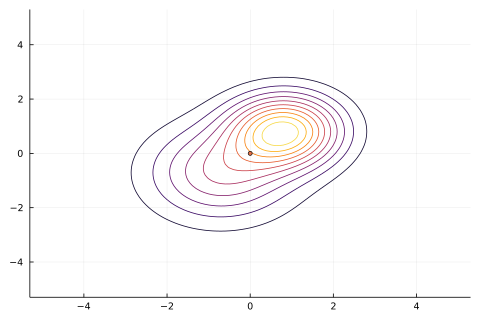
\includegraphics[width=\textwidth]{../plots/posterior/[0.1, 10.0].png}
        \caption{$\bar K_1 = 0.1, \bar K_2 = 10$}
        \label{fig:unimode}
    \end{subfigure}
    \hfill
    \begin{subfigure}{0.49\textwidth}
        \centering
        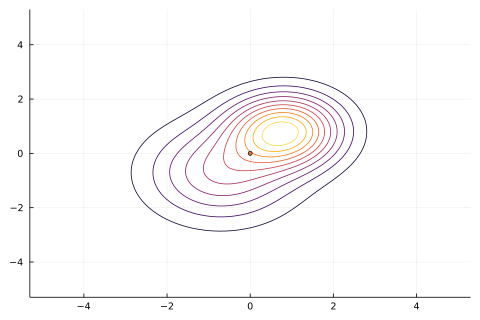
\includegraphics[width=\textwidth]{../plots/posterior/[10.0, 0.1].png}
        \caption{$\bar K_1 = 10, \bar K_2 = 0.1$}
        \label{fig:bimode}
    \end{subfigure}
    \caption{The posterior density $f \mid \eta=[0,0]$. The diagonals on the matrix $\Sigma_\eta$ are varied to demonstrate that the modal point varies dramatically with attention. State 2, the mode on the bottom of the figure, has twice the variance of state 1.}
    \label{fig:swapped}
\end{figure}


\section{Equilibrium}

\textcite{kacperczyk_rational_2016} work backwards by solving the portfolio allocation problem first, and then using this solution to determine the optimal information choice. I defer to their solution, though with some added complexity due to the change in the densities of $f$, $s$, and $p$ from multivariate Gaussians to mixture distributed variables.

\begin{maxi}
    {q_{j}}{U_{j2} = E_j[\exp{-\rho W_j} \mid \eta_j, p]}
    {\label{eq:learning-opt}}{}
    \addConstraint{W_j }{= r W_0 + q'_j (f - pr)}
\end{maxi}

\pagebreak
\appendix

\section{Mixture model variance}

The variance-covariance matrix of variable $X$ following a Gaussian mixture distribution with means $\mu = [\mu_1, \mu_2, \dots, \mu_k]'$, covariances $\Sigma= [\Sigma_1, \Sigma_2, \dots, \Sigma_k]$, and mixture proportions $\pi = [\pi_1, \pi_2, \dots, \pi_k]'$ is\footnote{From https://math.stackexchange.com/questions/195911/calculation-of-the-covariance-of-gaussian-mixtures} 

\begin{align}
    \Var[X] &= E[\Var[X \mid k]] + \Var[E[X \mid k]] \\
            &= \sum_k  \pi_k  \bigg(\Sigma_k + (\mu_k - \overline{\mu})(\mu_k - \overline{\mu})' \bigg)
\end{align}

\noindent for $\overline{\mu}=\sum_k \pi_k \mu_k$.

% \newpage
% \printbibliography

\end{document}
